\documentclass[a4paper]{article}
\usepackage{student}
\usepackage{graphicx,amsmath,booktabs,hyperref}
\hypersetup{colorlinks=true,urlcolor=blue}
\setmodule{Assignment 3 Report}
\setterm{115-1 (Fall 2026)}
\title{Reinforcement Learning}
\setmembername{Bo-Yu Lien}
\setmemberuid{b13901072}
\begin{document}
\header{}
\section{2048}
\begin{answer}[Q1. Monte Carlo evaluation]
I save 12 states visited by each greedy policy, $\pi(s)=\arg\max_a Q(s,a)$.
For each state, I take $a=\pi(s)$ and then follow the same policy until the game ends.
I repeat this 64 times, restoring the board, score and illegal-move counter each time.
Each rollout uses a different random seed. New tiles remain random: 2 with probability 0.9 and 4 with probability 0.1, at a random empty cell.
\[
G_j=\sum_{t=0}^{T_j-1}0.99^t r_t,\qquad
\widehat Q^\pi(s,a)=\frac{1}{64}\sum_{j=1}^{64}G_j.
\]
The 95\% confidence interval is $\bar G\pm1.998\,s_G/\sqrt{64}$, where $s_G$ is the sample standard deviation.
It describes randomness in future tiles for that fixed state.
No rollout reached the 2,000-step safety limit.
I use the training reward and termination rules here, so MC and the network estimate the same kind of return.
\end{answer}
\begin{answer}[Q2. DQN and DDQN: predicted Q versus MC Q]
Both comparison models were trained for 40,000 steps with seed 42 and the same network, reward and training settings. Only the Q target differs.
\begin{center}
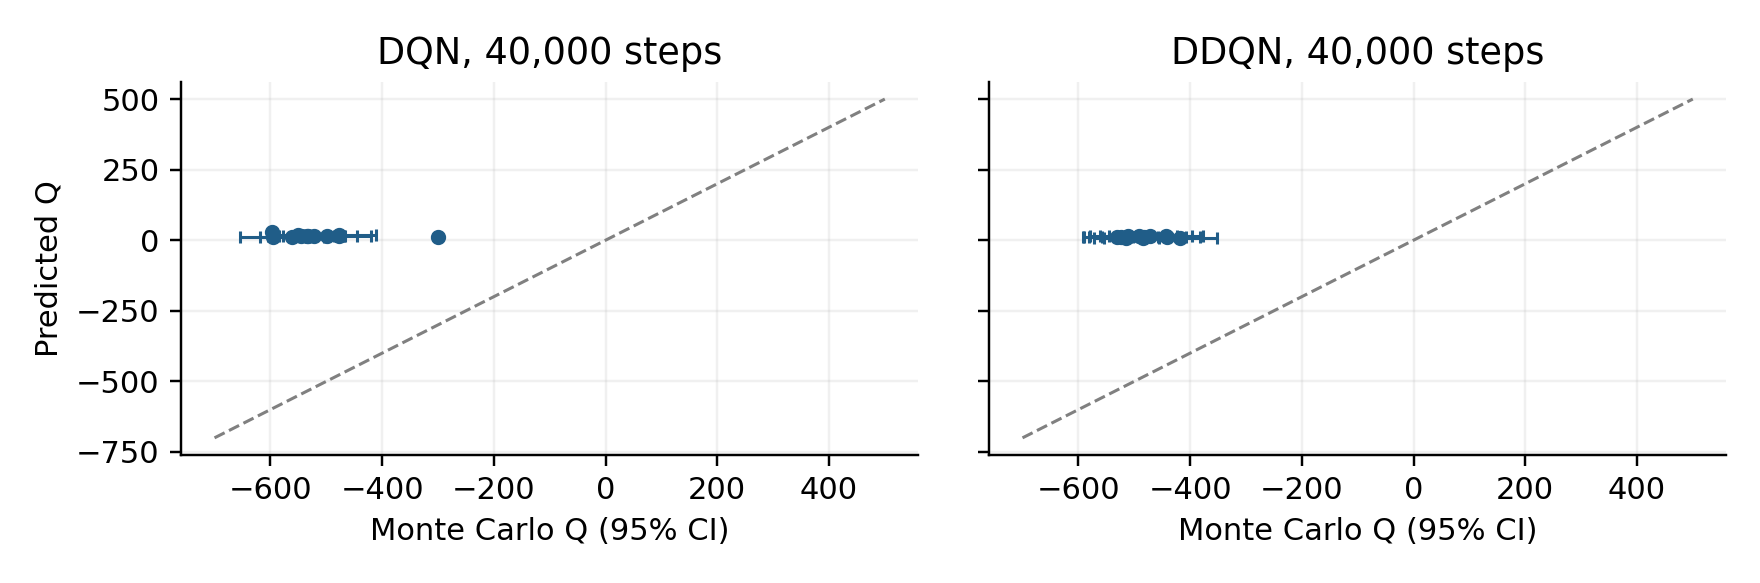
\includegraphics[width=.96\linewidth]{mc_comparison.png}
\end{center}
Each dot is one visited state. Bars show the 95\% MC interval; the dashed line is $Q=\widehat Q$.
The data come from the saved MC returns in \texttt{report\_work/results/mc\_dqn.json} and \texttt{mc\_ddqn.json}.

Both models overestimate these states. The mean $Q-\widehat Q$ is \textbf{531.6 for DQN} and \textbf{497.5 for DDQN}.
DQN uses the target network to both choose and evaluate the best next action.
DDQN chooses with the online network and evaluates with the target network. This can reduce overestimation caused by choosing an action with an accidentally high Q value.

DDQN has a smaller gap in this run, but each policy visits different states and only one training seed was tested.
A small gap does \emph{not} imply a good policy: a weak policy can correctly predict its own low return. Actual game scores must also be checked.
\end{answer}
\newpage
\begin{answer}[Q3. Best 2048 model]
I use DDQN with a one-hot board input ($16\times4\times4$), two 256-unit ReLU layers and four Q outputs.
The learning rate is $10^{-4}$, discount is 0.99, replay size is 100,000 and batch size is 256. Exploration decreases from $\epsilon=1$ to 0.05.
Training uses four environments and 20 blocks of 20,000 steps. After each block, the script checks ten games and saves when mean score or mean highest tile improves. The selected checkpoint has 360,000 steps.

A legal move gets its merge score plus the change in a weighted board sum. Larger weights near the lower-left corner encourage large tiles to stay together:
\[
r=\text{merge score}+\sum_{x,y}W_{x,y}(B'_{x,y}-B_{x,y}),\quad
W=\begin{bmatrix}0&0&0&0\\0.5&0&0&0\\0.75&0.5&0&0\\1&0.75&0.5&0\end{bmatrix}.
\]
Here $B'$ includes the new tile. An illegal move gives $-300$; three consecutive illegal moves end training episodes. Official testing ends at the first illegal move and uses the game score without shaping.
On public seeds 0--99, the saved model has mean score \textbf{1238.0} and best tile \textbf{512}.
\end{answer}
\section{Astro Party}
\begin{answer}[Q4. Best-model pipeline]
\textbf{Controller $\rightarrow$ imitation $\rightarrow$ PPO.}
The policy combines hand-written rules with learning. The rules also remain in the feature extractor during testing.
They aim ahead of the enemy, flee when my ship becomes a pilot, and chase an enemy pilot.
For bullet dodging, the controller predicts the next 60 steps and checks 15 turn/thrust choices when the planned move is unsafe. It checks the firing direction again after turning.

The input has 84 values. The extractor combines three controller actions with the first 26 input values.
A linear actor maps these 29 features to turn, thrust and shoot; the critic has two 64-unit Tanh layers.
I first train the actor to copy 10,000 teacher examples for 120 epochs using mean squared error and Adam with learning rate 0.003.

Then I fine-tune with PPO for \textbf{40,960 environment steps}, using seed 42 and four environments. Each episode randomly selects Rusher or Sniper with equal probability.
PPO uses learning rate $10^{-6}$, 512 rollout steps per environment, batch size 256, five update epochs, discount 0.995, GAE 0.95 and clip range 0.1.
Small action noise (initial log standard deviation $-3.5$) limits changes to the copied behavior. I use the last checkpoint.

The reward is $+20/-20$ for killing/dying, $+3/-3$ for enemy/own ejection, $+0.1$ for a pickup and $-0.002$ per step. Respawn and asteroid hits give zero.
Nonterminal steps also get $c(d_{\rm old}-d_{\rm new})$, with distance divided by 600: $c=-0.5$ when I am a pilot, 2 when only the enemy is a pilot, and 0.5 otherwise.

The saved public evaluation (100 games per opponent, seeds 0--99) gives \textbf{95\% against Rusher and 91\% against Sniper}. Draws count as failures. These seeds were used during development.
\end{answer}
\newpage
\begin{answer}[Q5. PPO versus A2C]
\textbf{Hypothesis.} Under the same short training budget, PPO will give a higher Sniper win rate than A2C after starting from the same imitation policy.
PPO limits policy changes through clipping and reuses each rollout, which may help keep useful aiming and dodging behavior.

\textbf{Experiment.} Both SB3 algorithms start with exactly the same actor and critic weights from the imitation checkpoint.
They use the same controller, reward, four environments, learning rate $10^{-6}$, discount 0.995, GAE 0.95 and 512-step rollouts.
Both use Adam, normalized advantages and \textbf{8,192 environment steps}.
PPO uses five update epochs with batch size 256; A2C updates once per rollout.

The experiment repeats with training rollout seeds 42, 43 and 44.
Each model is tested on the same 30 games per opponent (seeds 72000--72029), using deterministic actions and counting draws as failures.
\begin{center}
\begin{tabular}{lrrr}
\toprule
Rollout seed & PPO: Sniper & A2C: Sniper & Both: Rusher\\
\midrule
42 & 25/30 (83.3\%) & 22/30 (73.3\%) & 29/30 (96.7\%)\\
43 & 27/30 (90.0\%) & 23/30 (76.7\%) & 29/30 (96.7\%)\\
44 & 27/30 (90.0\%) & 22/30 (73.3\%) & 29/30 (96.7\%)\\
\midrule
Mean & 87.8\% & 74.4\% & 96.7\%\\
\bottomrule
\end{tabular}
\end{center}
Source: \texttt{report\_work/results/astro\_algorithm\_comparison.json}, including the individual game outcomes.

\textbf{Conclusion.} PPO beats A2C against Sniper in all three pairs, supporting the hypothesis for this setting. They tie against Rusher.
However, PPO performs more optimizer updates, so this test cannot show whether clipping or extra updates caused the difference.
All runs share one imitation checkpoint and the same test games. The result is about short fine-tuning, not learning from scratch or a universal advantage of PPO.
\end{answer}
\small
\textbf{Sources and assistance.}
Results are from the repository's saved experiments; the figure was redrawn from their raw returns.
Methods follow the provided game code, SB3 implementations and the Double DQN paper (van Hasselt et al., 2015).
AI assistance was used for code, experiments and editing. The accompanying source guide maps each result to its script and data.
\end{document}
